\graphicspath{
    {figures_and_references/EELISA_conference/}
}

% \selectlanguage{english}
\renewcommand{\chapternametext}{Chapter \thechapter: Seismic risk}

\begin{refsection}

\chapter{\chapternametext}
\

\renewcommand{\headingtextL}{}
\renewcommand{\headingtextR}{\chapternametext}
\begingroup
 \flushbottom
 \setlength{\parskip}{0pt plus 1fil}%
 \localtableofcontents 
\endgroup

\begingroup
 \flushbottom
 \setlength{\parskip}{0pt plus 1fil}%
 \locallistoffigures
 \locallistoftables
\endgroup


\newpage

\setcounter{section}{0} 



\FloatBarrier

\renewcommand{\sectionnametext}{Seismic Risk}
\renewcommand{\headingtextL}{\chapternametext}
\renewcommand{\headingtextR}{\thesection. \sectionnametext}
\section{\sectionnametext}

Seismic risk is defined as the product of three distinct components: hazard, exposure, and vulnerability. Expressed through the conceptual formula $Risk = Hazard \times Exposure \times Vulnerability$, this framework provides a comprehensive assessment of the potential losses that a city might sustain during an earthquake.

\textbf{Exposure} refers to the "elements at risk," encompassing the entire building stock, infrastructure, and population within a study area. In the context of urban seismic risk, the exposure component is captured through an inventory database, often a Geospatial Database, which contains individual records for each building. These records include essential attributes such as location, structural material, height, age, and occupancy, all of which are critical for characterizing the susceptibility of the assets.

\textbf{Vulnerability} is the inherent predisposition of the exposed elements to suffer damage or destruction when affected by a seismic event. As detailed in Section \ref{sec:seismic_vulnerability}, vulnerability is characterized through capacity curves, which measure a building's strength, and fragility curves, which provide the probabilistic distribution of damage states. These mathematical models allow for the translation of physical ground motion demand into tangible consequences, such as structural damage or economic loss.

\textbf{Hazard} represents the description of the seismic phenomenon itself. It encompasses the probability of a seismic event occurring in a specific region, along with its expected frequency, intensity, and ground-motion characteristics (such as peak acceleration or spectral ordinates). The hazard assessment deals with the natural source and propagation of energy, focusing on the seismic source zones and local soil effects. While hazard is the fundamental driver of seismic risk, it is important to note that the detailed estimation of hazard parameters, such as site-specific seismic source modelling or ground motion prediction equations, is out of the scope of this work.

By multiplying these components, the seismic risk assessment quantifies the expected consequences of future earthquakes. While hazard establishes the potential for ground motion, it is the integration with the inventory of the built environment (exposure) and its inherent mechanical resistance (vulnerability) that ultimately defines the level of danger faced by the city. This holistic approach is the foundation for effective disaster risk reduction, allowing decision-makers to identify the most critical sectors for retrofitting and to develop informed emergency response strategies.

\renewcommand{\sectionnametext}{Seismic exposure}
\renewcommand{\headingtextR}{\thesection. \sectionnametext}
\section{\sectionnametext}

Various taxonomies have been developed to identify main building attributes that influence seismic behaviour and therefore should be included in exposure databases. In 2012, the Global Earthquake Model (GEM) consortium introduced the GEM v2.0 taxonomy, aiming to overcome the limitations of previous classification systems \footcite{brzev_gem_2013}. Through a comparative analysis of ten existing schemes, a ranking was developed based on criteria such as simplicity, completeness, usability, and geographic applicability.


The GEM v2.0 taxonomy, validated by the Earthquake Engineering Research Institute (EERI), was designed to be both comprehensive and straightforward, user-friendly, and adaptable to other types of structures and natural hazards. It defines 13 attributes that influence the seismic performance of a building (tab. \ref{tab:GEM_attributes}) \footcite{brzev_gem_2013}: direction, material of the lateral load-resisting system (MLLRS) (structural material), lateral load-resisting system (LLRS) (type and system ductility), height, date of construction or retrofit, occupancy, building position within the block, shape of the building plan, structural irregularity, exterior walls, roof, floor and foundation. Some of these attributes have multiple classification levels.


\begin{table}[htbp]
\centering
\begin{tabular}{|l|l|l|l|}
\hline
\textbf{Group}                                                                          & \textbf{\#}         & \textbf{Attribute}                                                                                              & \textbf{Levels}                                                                    \\ \hline
\multirow{6}{*}{\begin{tabular}[c]{@{}l@{}}Structural \\ system\end{tabular}}           & 1                   & Direction                                                                                                       & Building direction                                                                 \\ \cline{2-4} 
    & \multirow{3}{*}{2}  & \multirow{3}{*}{\begin{tabular}[c]{@{}l@{}}Material of  the \\ lateral  load-\\resisting  system\end{tabular}} & Material type (level 1)                                                            \\ \cline{4-4} 
    &                     &                                                                                                                 & Material technology (level 2)                                                      \\ \cline{4-4} 
    &                     &                                                                                                                 & Material properties (level 3)                                                      \\ \cline{2-4} 
    & \multirow{2}{*}{3}  & \multirow{2}{*}{\begin{tabular}[c]{@{}l@{}}Lateral  load-\\resisting system\end{tabular}}                     & \begin{tabular}[c]{@{}l@{}}Type of lateral load-\\resisting system (level 1)\end{tabular}   \\ \cline{4-4} 
    &                     &                                                                                                                 & System ductility (level 2)                                                         \\ \hline
\multirow{4}{*}{\begin{tabular}[c]{@{}l@{}}Building \\ information\end{tabular}}        & 4                   & Height                                                                                                          & Height                                                                             \\ \cline{2-4} 
    & 5                   & \begin{tabular}[c]{@{}l@{}}Date of \\ construction \\ or retrofit\end{tabular}                                  & \begin{tabular}[c]{@{}l@{}}Year of construction \\ completion\end{tabular}         \\ \cline{2-4} 
    & \multirow{2}{*}{6}  & \multirow{2}{*}{Occupancy}                                                                                      & General (level 1)                                                                  \\ \cline{4-4} 
    &                     &                                                                                                                 & Detailed (level 2)                                                                 \\ \hline
\multirow{6}{*}{\begin{tabular}[c]{@{}l@{}}Exterior \\ attributes\end{tabular}}         & 7                   & \begin{tabular}[c]{@{}l@{}}Building position \\ within a block\end{tabular}                                     & \begin{tabular}[c]{@{}l@{}}Building position \\ within a block\end{tabular}        \\ \cline{2-4} 
    & 8                   & \begin{tabular}[c]{@{}l@{}}Shape of the \\ building plan\end{tabular}                                           & Footprint geometry                                                                 \\ \cline{2-4} 
    & \multirow{3}{*}{9}  & \multirow{3}{*}{\begin{tabular}[c]{@{}l@{}}Structural \\ irregularity\end{tabular}}                             & Regular or irregular (level 1)                                                     \\ \cline{4-4} 
    &                     &                                                                                                                 & \begin{tabular}[c]{@{}l@{}}Plan or vertical \\ irregularity (level 2)\end{tabular} \\ \cline{4-4} 
    &                     &                                                                                                                 & Type of irregularity (level 3)                                                     \\ \cline{2-4} 
    & 10                  & Exterior walls                                                                                                  & Exterior wall type                                                                 \\ \hline
\multirow{9}{*}{\begin{tabular}[c]{@{}l@{}}Roof, floors \\ and foundation\end{tabular}} & \multirow{5}{*}{11} & \multirow{5}{*}{Roof}                                                                                           & Roof shape (level 1)                                                               \\ \cline{4-4} 
    &                     &                                                                                                                 & Roof covering (level 2)                                                            \\ \cline{4-4} 
    &                     &                                                                                                                 & Roof system material (level 3)                                                     \\ \cline{4-4} 
    &                     &                                                                                                                 & Roof system type (level 4)                                                         \\ \cline{4-4} 
    &                     &                                                                                                                 & Roof connections (level 5)                                                         \\ \cline{2-4} 
    & \multirow{3}{*}{12} & \multirow{3}{*}{Floors}                                                                                         & Floor system material (level 1)                                                    \\ \cline{4-4} 
    &                     &                                                                                                                 & Floor system type (level 2)                                                        \\ \cline{4-4} 
    &                     &                                                                                                                 & Floor connections (level 3)                                                        \\ \cline{2-4} 
    & 13                  & Foundation system                                                                                               & Foundation system                                                                  \\ \hline
\end{tabular}
\caption{Attributes and classification levels according to GEM methodology.}
\label{tab:GEM_attributes}
\end{table}

\renewcommand{\sectionnametext}{Seismic vulnerability}
\renewcommand{\headingtextR}{\thesection. \sectionnametext}
\section{\sectionnametext}
\label{sec:seismic_vulnerability}

The seismic vulnerability of a structure is defined as its intrinsic predisposition to sustain damage during an earthquake of a given severity. As noted by \footcite{barbat_seismic_2010}, vulnerability encompasses the degree of damage, the lack of resilience, and the limited response capacity that components of a city may exhibit when exposed to probable seismic events throughout their lifecycle. Within earthquake engineering, various methodologies, categorized as empirical, analytical, or hybrid, have been developed to assess this vulnerability, primarily based on the structural performance of buildings relative to their construction typology \footcite{martinez-cuevas_urban_2014, yepes-estrada_modeling_2017}.

Vulnerability assessment relies on two fundamental instruments: capacity models and fragility models. A capacity model, or "pushover" curve, represents the non-linear force-displacement relationship of a structure by plotting base shear ($V$) against roof displacement ($\Delta_R$) (fig. \ref{fig:capacity_curve}. To facilitate the estimation of an expected performance point, this model is frequently converted into the Acceleration-Displacement Response Spectra (ADRS) format, yielding a capacity spectrum. This conversion integrates the structure's dynamic properties, such as its fundamental period ($T$), mode shapes, and effective mass.

\begin{figure}[htbp]
    \centering
    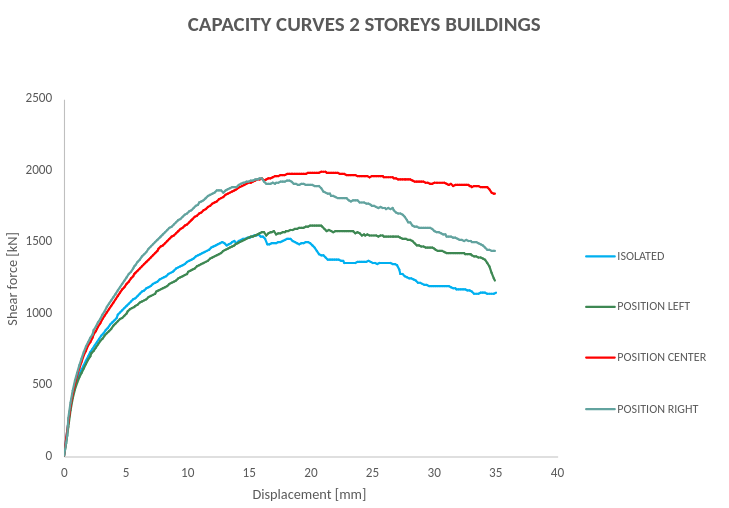
\includegraphics[width=0.6\linewidth]{figures/capacity_curve_1.png}
    \caption{Example of capacity curves depending on the relative position of the building within the block.}
    \label{fig:capacity_curve}
\end{figure}


Complementing these are fragility models, which provide a probabilistic assessment of damage \footcite{mouroux_presentation_2006,milutinovic_wp4_2003,barbat_seismic_2010,jimenez-martinez_methodology_2024}. These are often represented as a suite of fragility curves that define the conditional probability of a building reaching or exceeding specific damage states for a given level of spectral displacement ($S_d$). These curves are mathematically defined using the lognormal standard distribution, characterized by the median spectral displacement required to trigger a damage state and the associated lognormal standard deviation ($\beta$). Because the seismic response depends on variable material properties, construction quality, and the specific nature of ground motion, these models are developed within defined confidence intervals to account for inherent uncertainties.

The RISK-UE project \footcite{milutinovic_riskue_wp4_2003, mouroux_presentation_2006} formalizes this assessment through its Level II method (LM2), commonly known as the Capacity Spectrum Method. This approach evaluates seismic vulnerability by comparing the capacity spectrum of the structure under analysis against a site-specific demand spectrum. The method involves generating capacity and fragility curves for individual buildings or groups of buildings categorized by similar typological characteristics. These building typologies (BT) are generally defined using a combination of three key attributes: the material of the lateral load-resisting system (MLLRS), the type of lateral load-resisting system (LLRS), and the building height. Previous research identifies these as the most influential factors affecting seismic performance, though each contributes differently to overall vulnerability \footcite{jimenez-martinez_methodology_2024}.

In practice, every building typology must be assigned a corresponding capacity curve and a damage probability function. However, the final seismic response is also modulated by specific attributes known as "behaviour modifiers." While these are not part of the core typology definition, they exert a notable influence on the vulnerability of a structure, necessitating adjustments to the base capacity and fragility models to reflect the unique conditions of each building.

\renewcommand{\sectionnametext}{Behaviour modifiers}
\renewcommand{\headingtextR}{\thesection. \sectionnametext}
\section{\sectionnametext}


Behaviour modifiers are defined as a set of structural, constructive and urban planning attributes that influence the vulnerability of a building typology to earthquakes  \footcite{martinez-cuevas_urban_2017}. Their main function is to adjust the base vulnerability of a given building typology, acknowledging that the actual conditions of each structure can significantly increase or decrease its seismic response.


Behaviour modifiers are relevant in methodologies such as the RISK-UE project \footcite{milutinovic_riskue_wp4_2003}, considering factors such as the irregularities in plan or elevation, the location of the building within the aggregate, among others. For instance, in the case of the Lorca earthquake (Spain, 2011),  Tomás et al.\footcite{tomas_proposal_2017} demonstrate that properly accounting for behaviour modifiers helped reducing the discrepancy between observed and estimated damage.
These factors are not only useful for post-earthquake analysis, but also play a key role in preventive urban planning, as they help guide zoning regulations aimed at reducing urban risk, as proposed by Martínez-Cuevas et al. \footcite{martinez-cuevas_urban_2017}.

The modifiers that can be derived from building footprints are, among others, direction, plan irregularity, shape of the building plan and block position. This study focusses on these modifiers and proposes the integration of plan irregularity and shape of the building plan in a single modifier called the Footprint Shape Index (FSI).

\subsection{Direction}
This modifier allows users to describe the orientation of building(s) with different lateral load- resisting systems in two principal horizontal directions, which are assumed to be orthogonal to each other\footcite{brzev_gem_2013}. Different LLRS configurations and their corresponding MLLRS can be independently specified for each direction. Seismic vulnerability is typically evaluated in the most unfavourable direction. Therefore, the direction of ground-motion relative to the building plays a crucial role in the calibration of the capacity and fragility curves \footcite{zucconi_fragility_2022}.

\subsection{Building position within the block}

The seismic assessment of aggregated buildings, requires classifying each unit based on its position within the aggregate or block, as this greatly influences its structural response. Based on existing research, buildings can be typified as isolated, corner, edge or central units. This classification provides a framework for identifying specific vulnerability patterns and guiding effective retrofitting strategies.

Isolated units, which are not physically connected to any neighbouring building, behave independently under seismic action. Comparative studies have shown that these structures tend to exhibit a higher probability of damage than those embedded within aggregates, mainly due to the absence of confining effects from adjacent buildings \footcite{chieffo_comparative_2019}

Corner units have been identified as particularly vulnerable. Research has revealed high concentrations of shear stresses in these locations, both in numerical simulations and in experimental studies \footcite{Battaglia2021, formisano_quick_2010}. These units also show asymmetric behaviour due to unilateral exposure to lateral loads.

Edge units are located at the ends of row configurations. They remain susceptible to torsional effects and differential displacements resulting from interactions with adjacent structures of differing mass or stiffness \footcite{Battaglia2021, valente_historical_2019}.

Central units, enclosed by neighbouring buildings on both sides, often benefit from the mass and confinement effects of the ensemble. As such, they usually experience smaller relative displacements. However, studies have shown that smaller internal units can suffer a significant reduction in damage due to interaction with larger adjacent buildings \footcite{greco_seismic_2020}.

Recent literature also emphasises the importance of accounting for structural interactions and pounding effects between adjacent units \footcite{angiolilli_seismic_2021}, as well as boundary conditions and connection quality, aspects that remain underexplored in numerical modelling. Even in modern aggregates, such as partially grouted reinforced concrete masonry (PG-RCM), differences in seismic behaviour have been observed depending on the position of each unit \footcite{torres-olivares_seismic_2024, torres-olivares_numerical_2025}
In the present study, this classification is derived from the digitised footprint geometry. Consequently, it assumes that each mapped footprint represents a single structural unit, unless separation between adjacent units is clearly visible and can be digitised independently.



\subsection{Structural irregularity} %propongo este esquema pero hay que poner las citas y las normativas
The irregular configuration either in plan or elevation is recognised as one of the main causes of failure during earthquakes \footcite{brzev_gem_2013}, \footcite{naveen_analysis_2019}. An analysis of 21 significant seismic events that occurred between 1980 and 2003 revealed a strong correlation between the severity of structural damage and the presence of irregularities in the configurations of buildings \footcite{raul_gonzalez_herrera_influence_2008}.  These asymmetric configurations, which result from irregular distributions of mass and stiffness or specific shapes in the plan or elevation, significantly affect the dynamic behaviour of buildings, particularly in terms of lateral displacements, torsion, and stress concentrations.

Based on the building footprint, plan irregularity is the only attribute that can be directly quantified. In this context, the analysis is necessarily limited to the external footprint geometry and does not explicitly account for seismic or expansion joints, or for internal subdivision into structurally independent units, unless these are evident in the mapped footprint.
Within this category, the present study focusses specifically on the shape of the building footprint and eccentricity, which have been extensively discussed in the technical literature. The shape of the building footprint refers to the effects caused by re-entrant corners or setbacks. These are common in buildings with 'L', 'T', 'U', 'X', or 'H' shape, and will be addressed in detail in the following subsection. Eccentricity arises when the centre of mass does not coincide with the centre of stiffness, leading to undesirable rotational movements. The resulting torsion depends on the degree of eccentricity and can significantly amplify the building’s seismic response \footcite{gokdemir_effects_2013}

\subsection{Shape of the building footprint} %propongo este esquema pero hay que poner las citas y las normativas

The factors derived from the shape of the building footprint encompass both the geometric layout (compactness), slenderness and eccentricity. All codes include shape irregularity indexes, some of them simplified depending on the level of irregularity.  The geometric configuration is associated with irregularities caused by setbacks, which are typical in buildings with 'L', 'T', 'U' or 'H', shapes. These configurations lead to stress concentrations at the internal corners, which are particularly susceptible to localised damage or early structural failure during seismic events \footcite{naveen_analysis_2019}. Additionally, they may give rise to unforeseen torsional effects.

The slenderness, defined as the ratio between the length and width of the building, plays an important role in its dynamic response. Structures with overly elongated or narrow floor plans tend to exhibit increased differential displacements when subjected to seismic loading.

Several approaches have been applied to quantify shape compactness, as  the convexity index, calculated as the ratio between the area within the circumscribed polygon and the area of the footprint itself \footcite{sarabandi_building_2008, ji_fully_2019}. Other authors employ the Polsby-Popper index, that compares footprint area and that of the the circumscribing circle \footcite{polsby_third_1991}. Polsby-Popper index compares the relationship between the area and the perimeter of a footprint to that of a circle. Higher values indicate more compact shapes, while lower values reflect greater irregularity. Its straightforward formulation has made it suitable for large-scale applications in the assessment of footprint geometry and its potential influence on seismic vulnerability \footcite{torres_using_2023}.

Accordingly, the shape-related attributes considered in this work refer to the apparent external footprint and may differ from the actual structural configuration when multiple independent units are aggregated within a single mapped outline.

Although shape and irregularity are discussed separately here for consistency with the GEM taxonomy, in the proposed methodology their footprint-related effects are combined into the integrated Footprint Shape Index (FSI).

\newpage

\renewcommand{\sectionnametext}{References}
\renewcommand{\headingtextR}{\thesection. \sectionnametext}
\section{\sectionnametext}
\printbibliography[heading=none]

\end{refsection}